\chapter*{Proposition 3}
\label{prop:3}

\begin{figure*}[ht]
    \begin{center}
    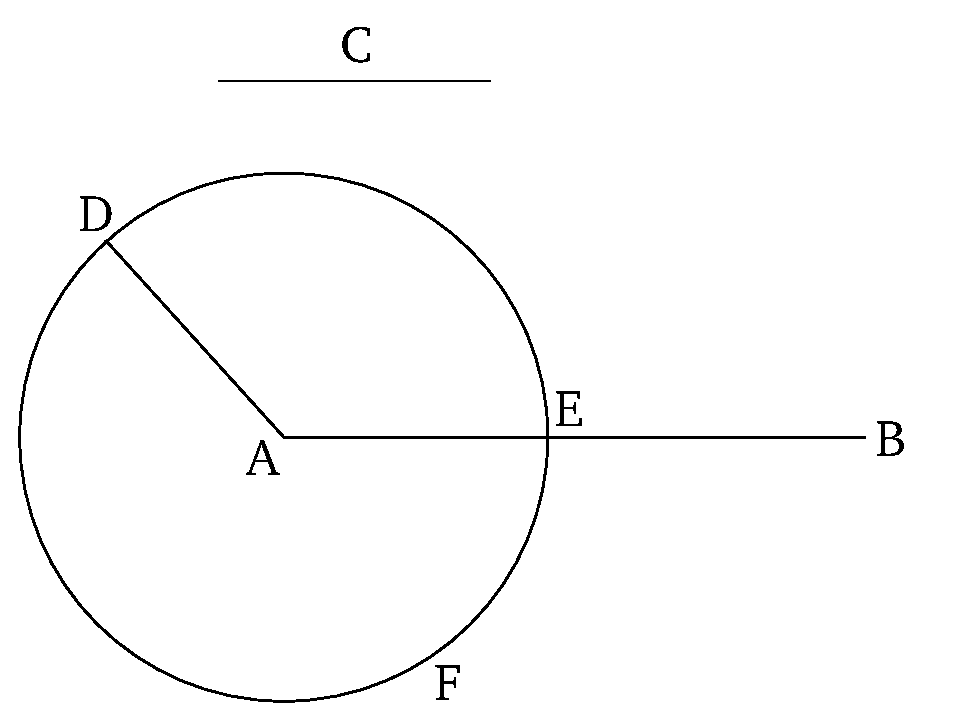
\includegraphics[width=0.5\linewidth]{figures/fig03e.eps}
    \label{fig:prop_3}
    \end{center}
\end{figure*}

For two given unequal straight-lines, to cut off from the greater a straight-line
equal to the lesser.

Let $AB$ and $C$ be the two given unequal straight-lines, of which let the greater be $AB$. So it is required to cut off a straight-line equal to the lesser $C$ from the greater $AB$.

Let the line $AD$, equal to the straight-line $C$, have been placed at  point $A$ [Prop.~1.2]. And let
the circle $DEF$ have been drawn with center $A$ and radius $AD$ [Post.~\ref{post:3}].

And since  point $A$ is the center of  circle $DEF$, $AE$ is equal to $AD$ [Def.~\ref{def:5}]. But,
$C$ is also equal to $AD$. Thus, $AE$ and $C$ are each equal to $AD$. So $AE$
is also equal to $C$ [C.N.~\ref{cn:1}].

Thus, for two given unequal straight-lines, $AB$ and $C$, the (straight-line) $AE$, equal to
the lesser $C$, has been cut off from the greater $AB$. (Which is) the very thing it was required to do.

\section*{Commentary}

\begin{proposition}\label{proposition_3}\lean{Elements.Book1.proposition_3}\leanok
   $A$ and $B$ are two distinct points on a line $AB$. $C_0$ and $C_1$ are two distinct points on a line $C$. $A \neq C_0$, and $|AB| > |C_0C_1|$. There must be a point $E$ between $A$ and $B$, s.t., $|AE| = |C_0C_1|$
\end{proposition}
\begin{proof}
    \uses{proposition_3}\leanok
    See the original proof by Euclid.
\end{proof}
